\chapter{Spatially entangled 4-photons states from a periodically poled KTP crystal}

\framebox[\textwidth]{
\begin{minipage}[b]{.75\textwidth}
\vskip 0.5em
The contents of this chapter serve as an example and are based on a scientific paper published as Phys. Rev. A {\bf 85}, 043837 (2012). This article contains results from the master thesis of Alexander J.H. van der Torren. The results and data analysis of the original master theses have been reproduced, extended and improved by S. Cigdem Yorulmaz at a later stage.
\vskip 0.5em
\end{minipage}
}

\vskip 2em

Photon pairs produced via spontaneous parametric down-conversion (SPDC) in a non-linear crystal give rise to strong nonclassical correlations. The resulting entangled photons are an important resource in quantum information, fundamental tests of quantum mechanics and have been used in experiments that demonstrate the violation of Bell's inequality, quantum teleportation and quantum communication. While most experiments focus on discrete polarization entanglement, quantum states of two particles that are entangled in continuous variables~\cite{Braunstein:RMP2005} such as frequency~\cite{Ou1988,Li2009}, time-bin~\cite{Friberg1985,Ou1999,Riedmatten2004} or photon momenta~\cite{Strekalov1995,Law2004,Howell2004,Walborn2010} are also possible, which gives access to high-dimensional entanglement that can be explored by measuring correlations between two photons.

In this article, we focus on spatial entanglement using photon momenta as a continuous variable. Unlike other forms of continuous variable entanglement, the quantum correlations in spatial entanglement can be resolved with relative ease and high resolution by using a combination of lenses and apertures only. The low conversion efficiency in non-linear crystals combined with the long coherence time of a continuous wave pump and ultrashort coherence time of the photon pairs ensure that most experiments are well described by two-photon interference of individual pairs~\cite{Walborn2010}. As a consequence, spatial entanglement with more than two photons has remained elusive and spatial correlations beyond independent photon pairs have not been addressed in an experiment~\cite{Assis2011}. These multi-photon states are of interest since they provide access to non-trivial entanglement between more than two particles~\cite{Greenberger1989,Dur2000}. Furthermore, the generation rate of four photon states sets fundamental limits on the visibility achievable in two-photon interference experiments~\cite{Marcikic2002} and the maximum attainable key generation rate in quantum key distribution protocols.

Here we investigate events where four spatially entangled photons are generated by SPDC. These four photons can either be two independent pairs, or they may all be in the same set of spatial and temporal modes to create a true four-photon state~\cite{Ou1999,Riedmatten2004}. The production of these four photon states is enhanced by the physical process of stimulated emission of a second photon pair into the same optical mode as the first pair. In the ideal situation of a single temporal and spatial mode, stimulated emission enhances the pair production rate by a factor of two compared to the probability to generate four photons in the same mode via two independent spontaneous processes. For a multi-mode situation, the relative importance of the stimulated emission process is given by a ``visibility'' $\chi$ that ranges from 0 to 1.

The distinction between two independent pairs and four-photon states has been addressed in the time-domain using time-bin entanglement with a pulsed laser source~\cite{Ou1999,Riedmatten2004}. These experiments are restricted to a single spatial mode and therefore do not allow use of spatial degrees of freedom to explore the process of stimulated emission. The total number of modes is then given by the available temporal modes and is directly related to the frequency bandwidth of the SPDC light as compared to the frequency bandwidth of the pulsed laser source~\cite{Riedmatten2004}. To directly resolve the underlying mode structure requires a measurement of quantum correlations within a single laser pulse. Such a direct measurement of the arrival time would require detectors with high quantum efficiency and sub-picosecond timing resolution, which is well outside reach of current single-photon detector technology~\cite{Hadfield2009,Eisaman2011}. Instead, we use spatially entangled multi-photon states that allow us to resolve the fine structure of stimulated pairs emitted in a single laser pulse in a straightforward way. Using pinholes the momentum resolution in the far-field of the SPDC source may be made arbitrarily high. In an experiment, there is always a trade-off between the size of the pinhole and the collected signal, which sets the time required to measure coincidence rates to a sufficient level of accuracy.

\section{Stimulated emission of spatially entangled 4-photon states}

The downconversion process in the PPKTP crystal that generates photon pairs in $N$ spatial modes can be described by an interaction Hamiltonian of the SPDC process given by~\cite{Simon2000,Kok2000}:
\begin{equation}
H = \kappa \sum_{i}^N a^\dagger_{\vec{q_i}} a^\dagger_{\vec{-q_i}} + \mathrm{h.c.},
\end{equation}
where $a^\dagger_{\vec{q_i}}$ is the creation operator that creates a single photon in a spatial mode labeled by the transverse wavevector $\vec{q_i}$. The operator $a^\dagger_{\vec{q_i}} a^\dagger_{\vec{-q_i}}$ thus creates a pair of photons that is correlated in their transverse photon momenta and forms the basis for spatial entanglement. The parameter $\kappa$ describes the strength of the non-linear interactions and contains, among others, the (time-dependent) field of the pump and the effective non-linearity of the PPKTP crystal. For our purpose, where we pump the crystal with an intense pulsed laser, $\kappa$ can be assumed to be a classical  quantity. The corresponding wavefunction of the state generated by SPDC can be directly obtained from the Hamiltonian:
$$
\ket{\Psi} = \exp(-i H \frac{t}{\hbar}) \ket{0} \approx (1-\frac{i t}{\hbar} H - \frac{t^2}{2 \hbar^2} H^2) \ket{0},
$$
where we limited the Taylor expansion in the last step to exclude quantum states with more than 4 photons. The linear term in the Taylor expansion creates a state $\ket{\Psi_2}$ that consists of a superposition of a single photon pair in any of the available spatial modes:
$$
\ket{\Psi_2} = \frac{- i t}{\hbar}H \ket{0} = \frac{- i \kappa t}{\hbar} \sum_{i=1}^N \ket{1_{\vec{q_i}};1_{\vec{-q_i}}}.
$$
Please note that we use a shorthand notation in which we leave out all spatial modes without a photon. The spatial modes that contain photons are numbered by the number of photons in that mode and the subscript refers to the transverse photon momentum of that mode. The quadratic term gives rise to a state $\ket{\Psi_4}$ with 4 photons that contains all double pair contributions, which can be represented using the same notation~\cite{Riedmatten2004} as
\begin{eqnarray*} \ket{\Psi_4} & = & \frac{- \kappa^2 t^2}{2 \hbar^2} \bigg( 2 \sum_{i=1}^N \ket{2_{\vec{q_i}};2_{\vec{-q_i}}} + \\ & & \sum_{i=1}^N \sum_{j=1, i \neq j}^{N} \ket{1_{\vec{q_i}},1_{\vec{q_j}};1_{\vec{-q_i}},1_{\vec{-q_j}}} \bigg).
\end{eqnarray*}
The effect of stimulated emission follows directly from the creation operators and is contained in the extra factor $\sqrt{2}$ when two photon pairs are created in the same spatial mode.

A measurement of a single photon in a particular spatial mode with wavevector $\vec{q_i}$ determines the wavevector of the twin photon and corresponds to a state projection: $a_{\vec{q_i}}\ket{\Psi}$. The state projection allows us to calculate the probabilities of creating a single photon pair $P_2$ as well as the probability $P_4$ to create a state with 4 photons in the same mode. For a single spatial and temporal mode, the probability $P_4$ is exactly equal to $P_2^2$ and is thus enhanced by a factor 2 compared to stimulated emission of two photon pairs in the same spatial modes. In a situation with more than one spatial mode, which is of interest here, stimulated emission enhances the probability $P_4$ by a factor $(1+\chi)$, where $\chi$ is a ``visibility'' from 0 to 1 that quantifies the extra contribution to the 4 photon states due to stimulated emission. The probability to create a 4 photon state with the photons in the same mode can then be expressed as~\cite{Riedmatten2004}:
\begin{equation}
P_4 = \frac{P_2^2}{2} (1+\chi).
\end{equation}

\section{Experimental investigation of 4-photon quantum correlations}

\subsection{Experiment}

\begin{figure}[tbp]
\centering 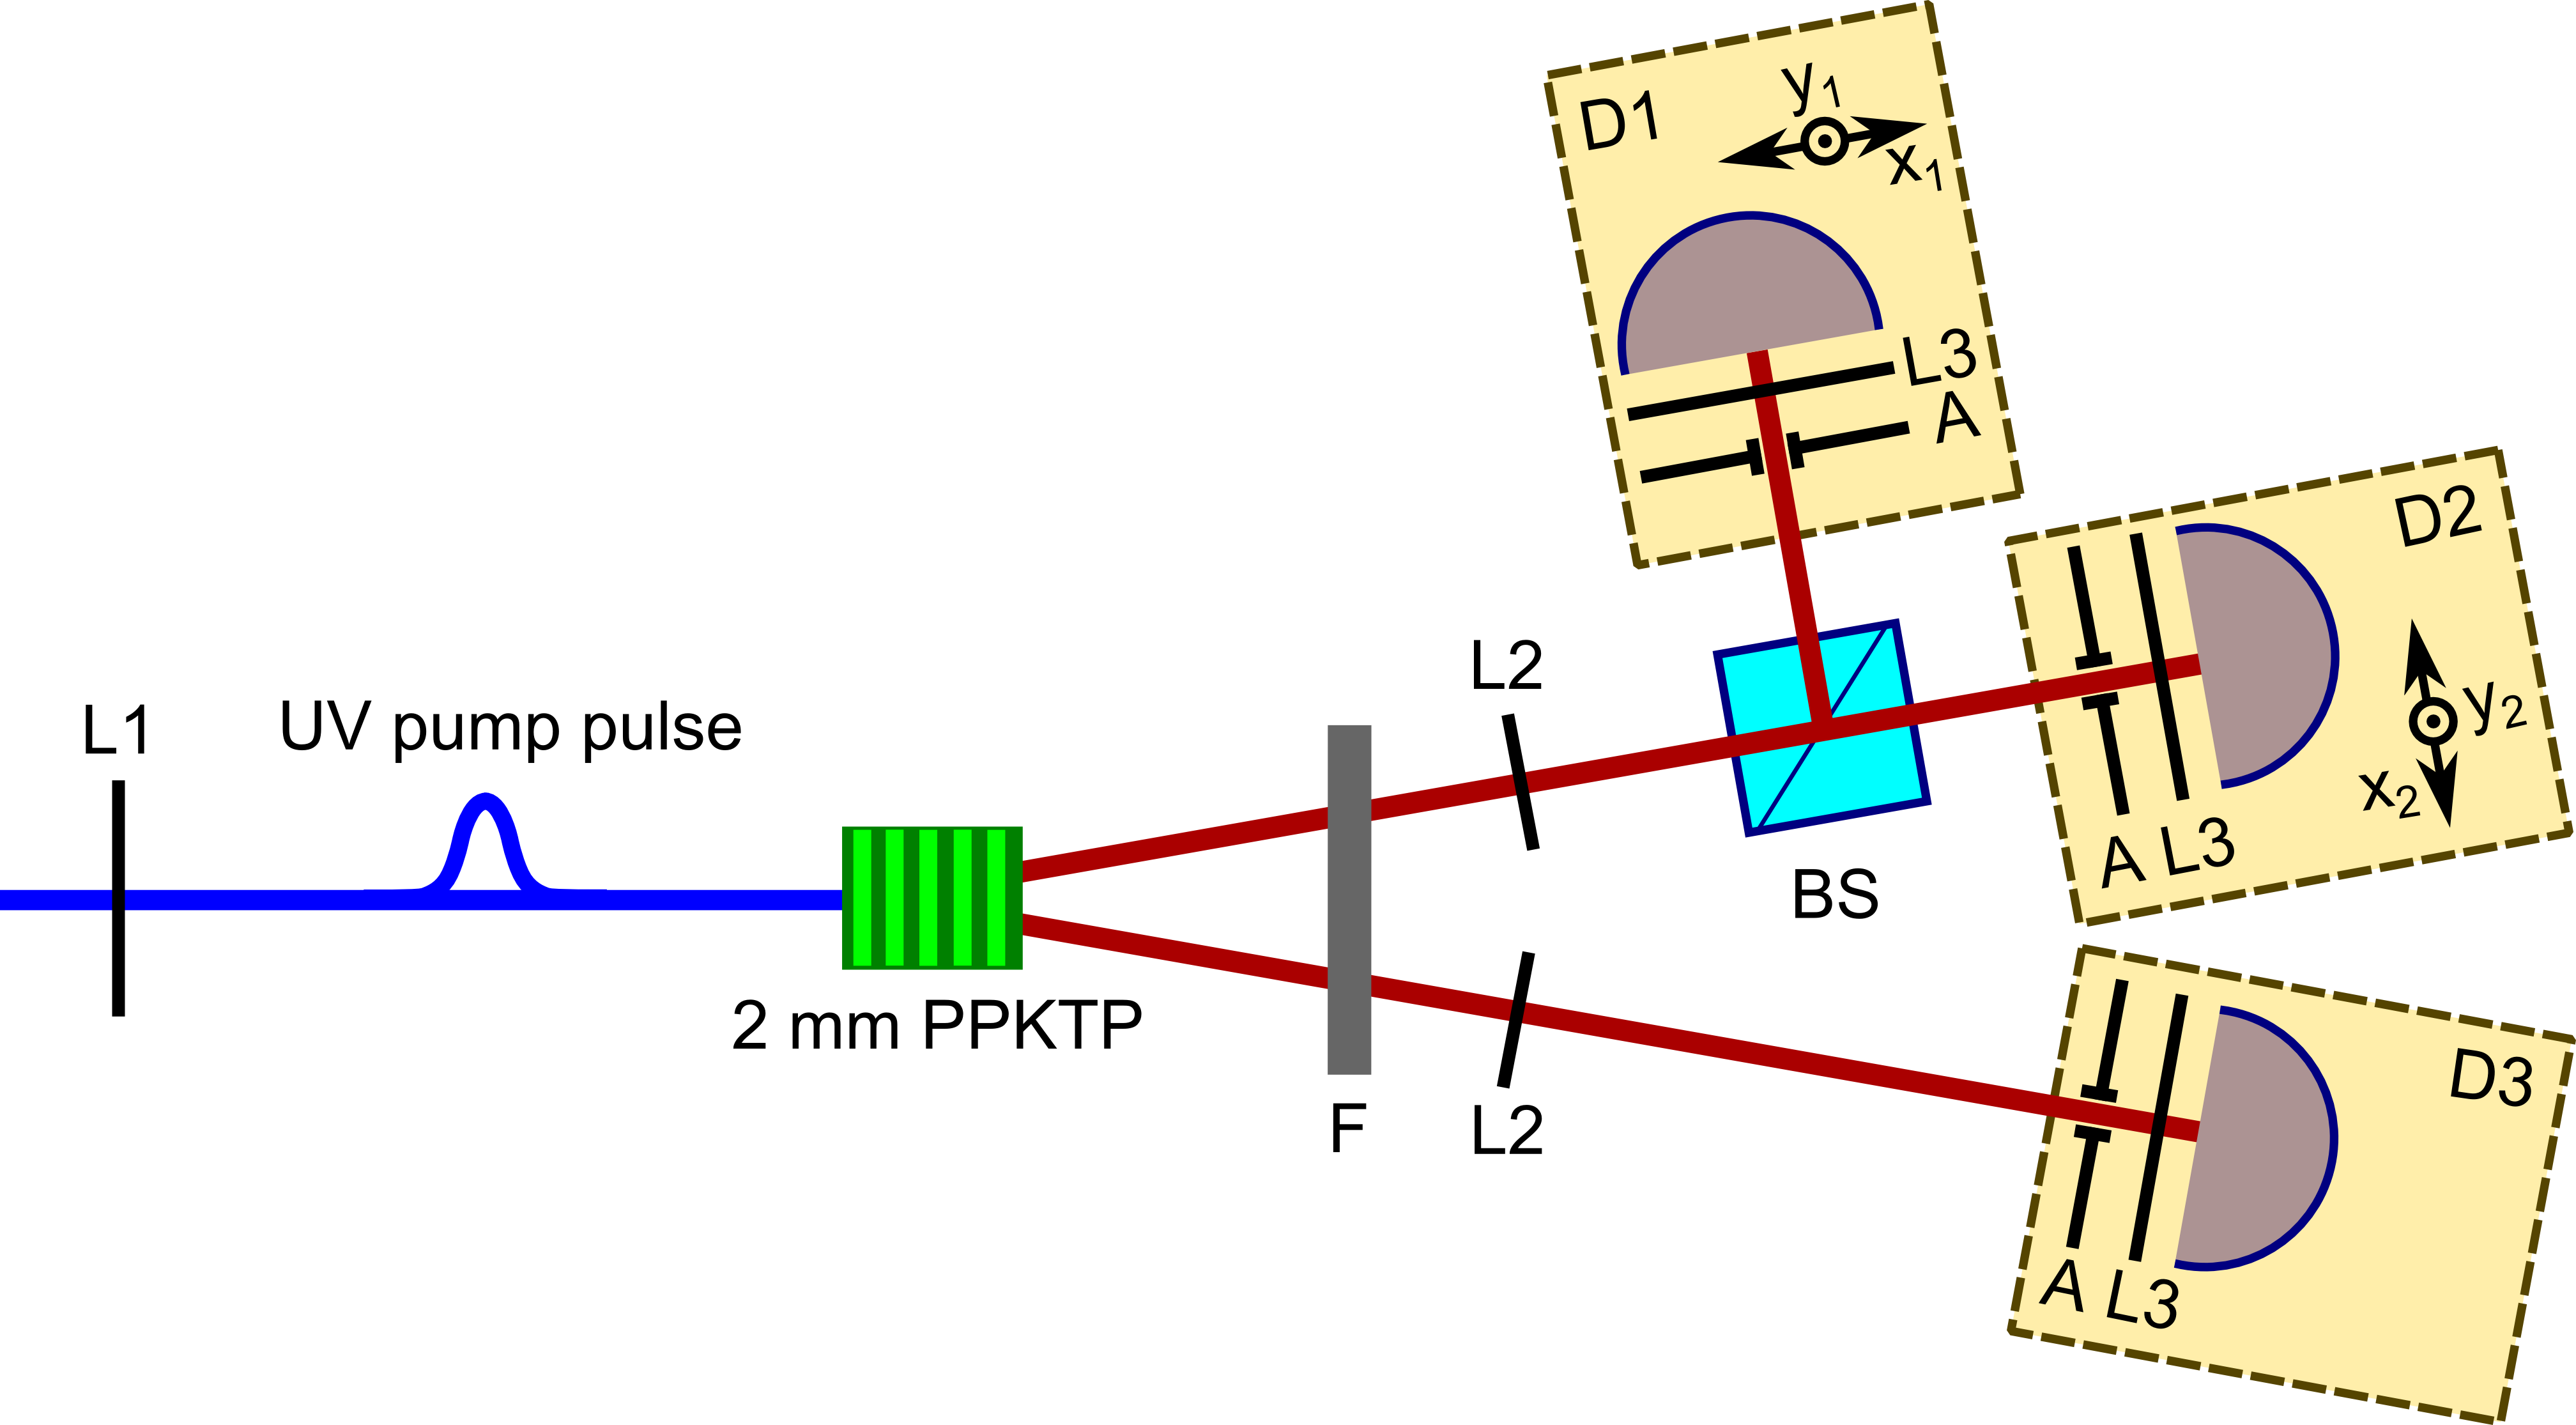
\includegraphics[width=120mm]{Fig1.png}
\caption{(Color online) Setup to measure spatially entangled 4-photon states via parametric downconversion in a 2 mm PPKTP crystal. UV pump pulses from a frequency doubled Ti:Sapphire laser are focused by lens L1 ($f_1$~=~250~mm). Photons are collected by the lenses $L2$ ($f_2$~=~270~mm) and detected by the detector assemblies $D1-D3$ that use photon counting APDs to detect single photons in a particular direction defined by the apertures $A$ placed in the combined focal planes of $L2$ and $L3$ ($f_3$~=~4.5~mm). The beamsplitter, $BS$, allows to record if two photons are in the same spatial mode. To this end detector assemblies $D1$ and $D2$ are placed on computer controlled translation stages. Correlations in the coincidence events are due to 4-photon states that are created by the process of stimulated emission of photon pairs.} \label{Fig:setup}
\end{figure}

Figure~\ref{Fig:setup} depicts the setup to explore the spatial quantum correlations due to stimulated emission of pairs in a four-photon state. In order to get a non-negligible rate of double pairs we use a highly efficient, 2 mm long, periodically poled KTP (PPKTP) crystal~\cite{Peeters2008} pumped by $\sim$100 mW of 413.2 nm pulsed laser light. The pulsed laser in our setup produces 2 ps pulses and is focussed into the PPKTP crystal using a lens $L1$, with a focal length $f$ of 250~mm. The source creates non-colinear, frequency degenerate photon pairs at a wavelength of 826.4 nm that are filtered by a bandpass filter $F$ and collected by lenses $L2$ ($f$~=~270~mm). Three detector assemblies $D1-D3$ are used to collect single photons with a well-defined momentum. Each of these assemblies consists of a lens $L3$ ($f_3$~=~4.5~mm), an aperture $A$ placed in the far-field to select the photon momentum and a (multi-mode) fiber-coupled single photon counting avalanche photodiode (Perkin-Elmer SPCM-AQ4C). The mode diameter of the fiber used in the experiments is $50$~$\mu$m and lenses $L2$ and $L3$ provide a 60$\times$ magnification factor. Coincidence detection with a $\sim$1.7~ns coincidence window between the detectors $D1$ and $D3$ (or $D2$ and $D3$) results in a measurement of spatial entanglement of single pairs. The beamsplitter, $BS$, allows us to record coincidence events between detectors $D1$ and $D2$ that are due to two photons from different pairs. To record the spatial correlations both detector assemblies $D1$ and $D2$ are placed on computer controlled translation stages that allow movement in the $x$ and $y$ directions transverse to the optical beam.

The essential feature of the setup is that it allows us to distinguish a genuine 4-photon state from two independent pairs by detecting coincidences between two photons in the same arm, as was introduced earlier for 4-photon states in the time-domain~\cite{Riedmatten2004}. In this setup only the 4-photon states created by stimulated emission generate strong correlations between detectors $D1$ and $D2$, while double pair states do not create any special correlations.

The length of the 2~ps laser pulse is a compromise between a short laser pulse to select a single temporal mode on the one hand and a somewhat longer laser pulse to retain efficient SPDC on the other hand. For a very short laser pulse the photons are created at a well-defined time, but the SPDC process becomes inefficient due to the broad spectral content of the laser pulse. In our study, the combination of the pulse duration and the bandpass filter selects $\sim$3 temporal modes, leading to a maximum possible visibility $\chi$=0.5 for a single spatial mode. The choice of the pulse duration and the length of the crystal was motivated by the group velocity walk-off length $L_g$ = 1.5 mm, calculated for transform-limited pulses, being comparable to the crystal length. Under those conditions, the phase-matching in the crystal is only mildly affected by the pulsed laser and all frequency components of the laser pulse contribute to the efficient generation of SPDC light.

% I calculated the GV walk-off length as \tau/|D|, with d=0.4/c and \tau=2 ps.

\subsection{Quantum correlations at the two-photon level and number of Schmidt modes}

\begin{figure}[tbp]
\centering 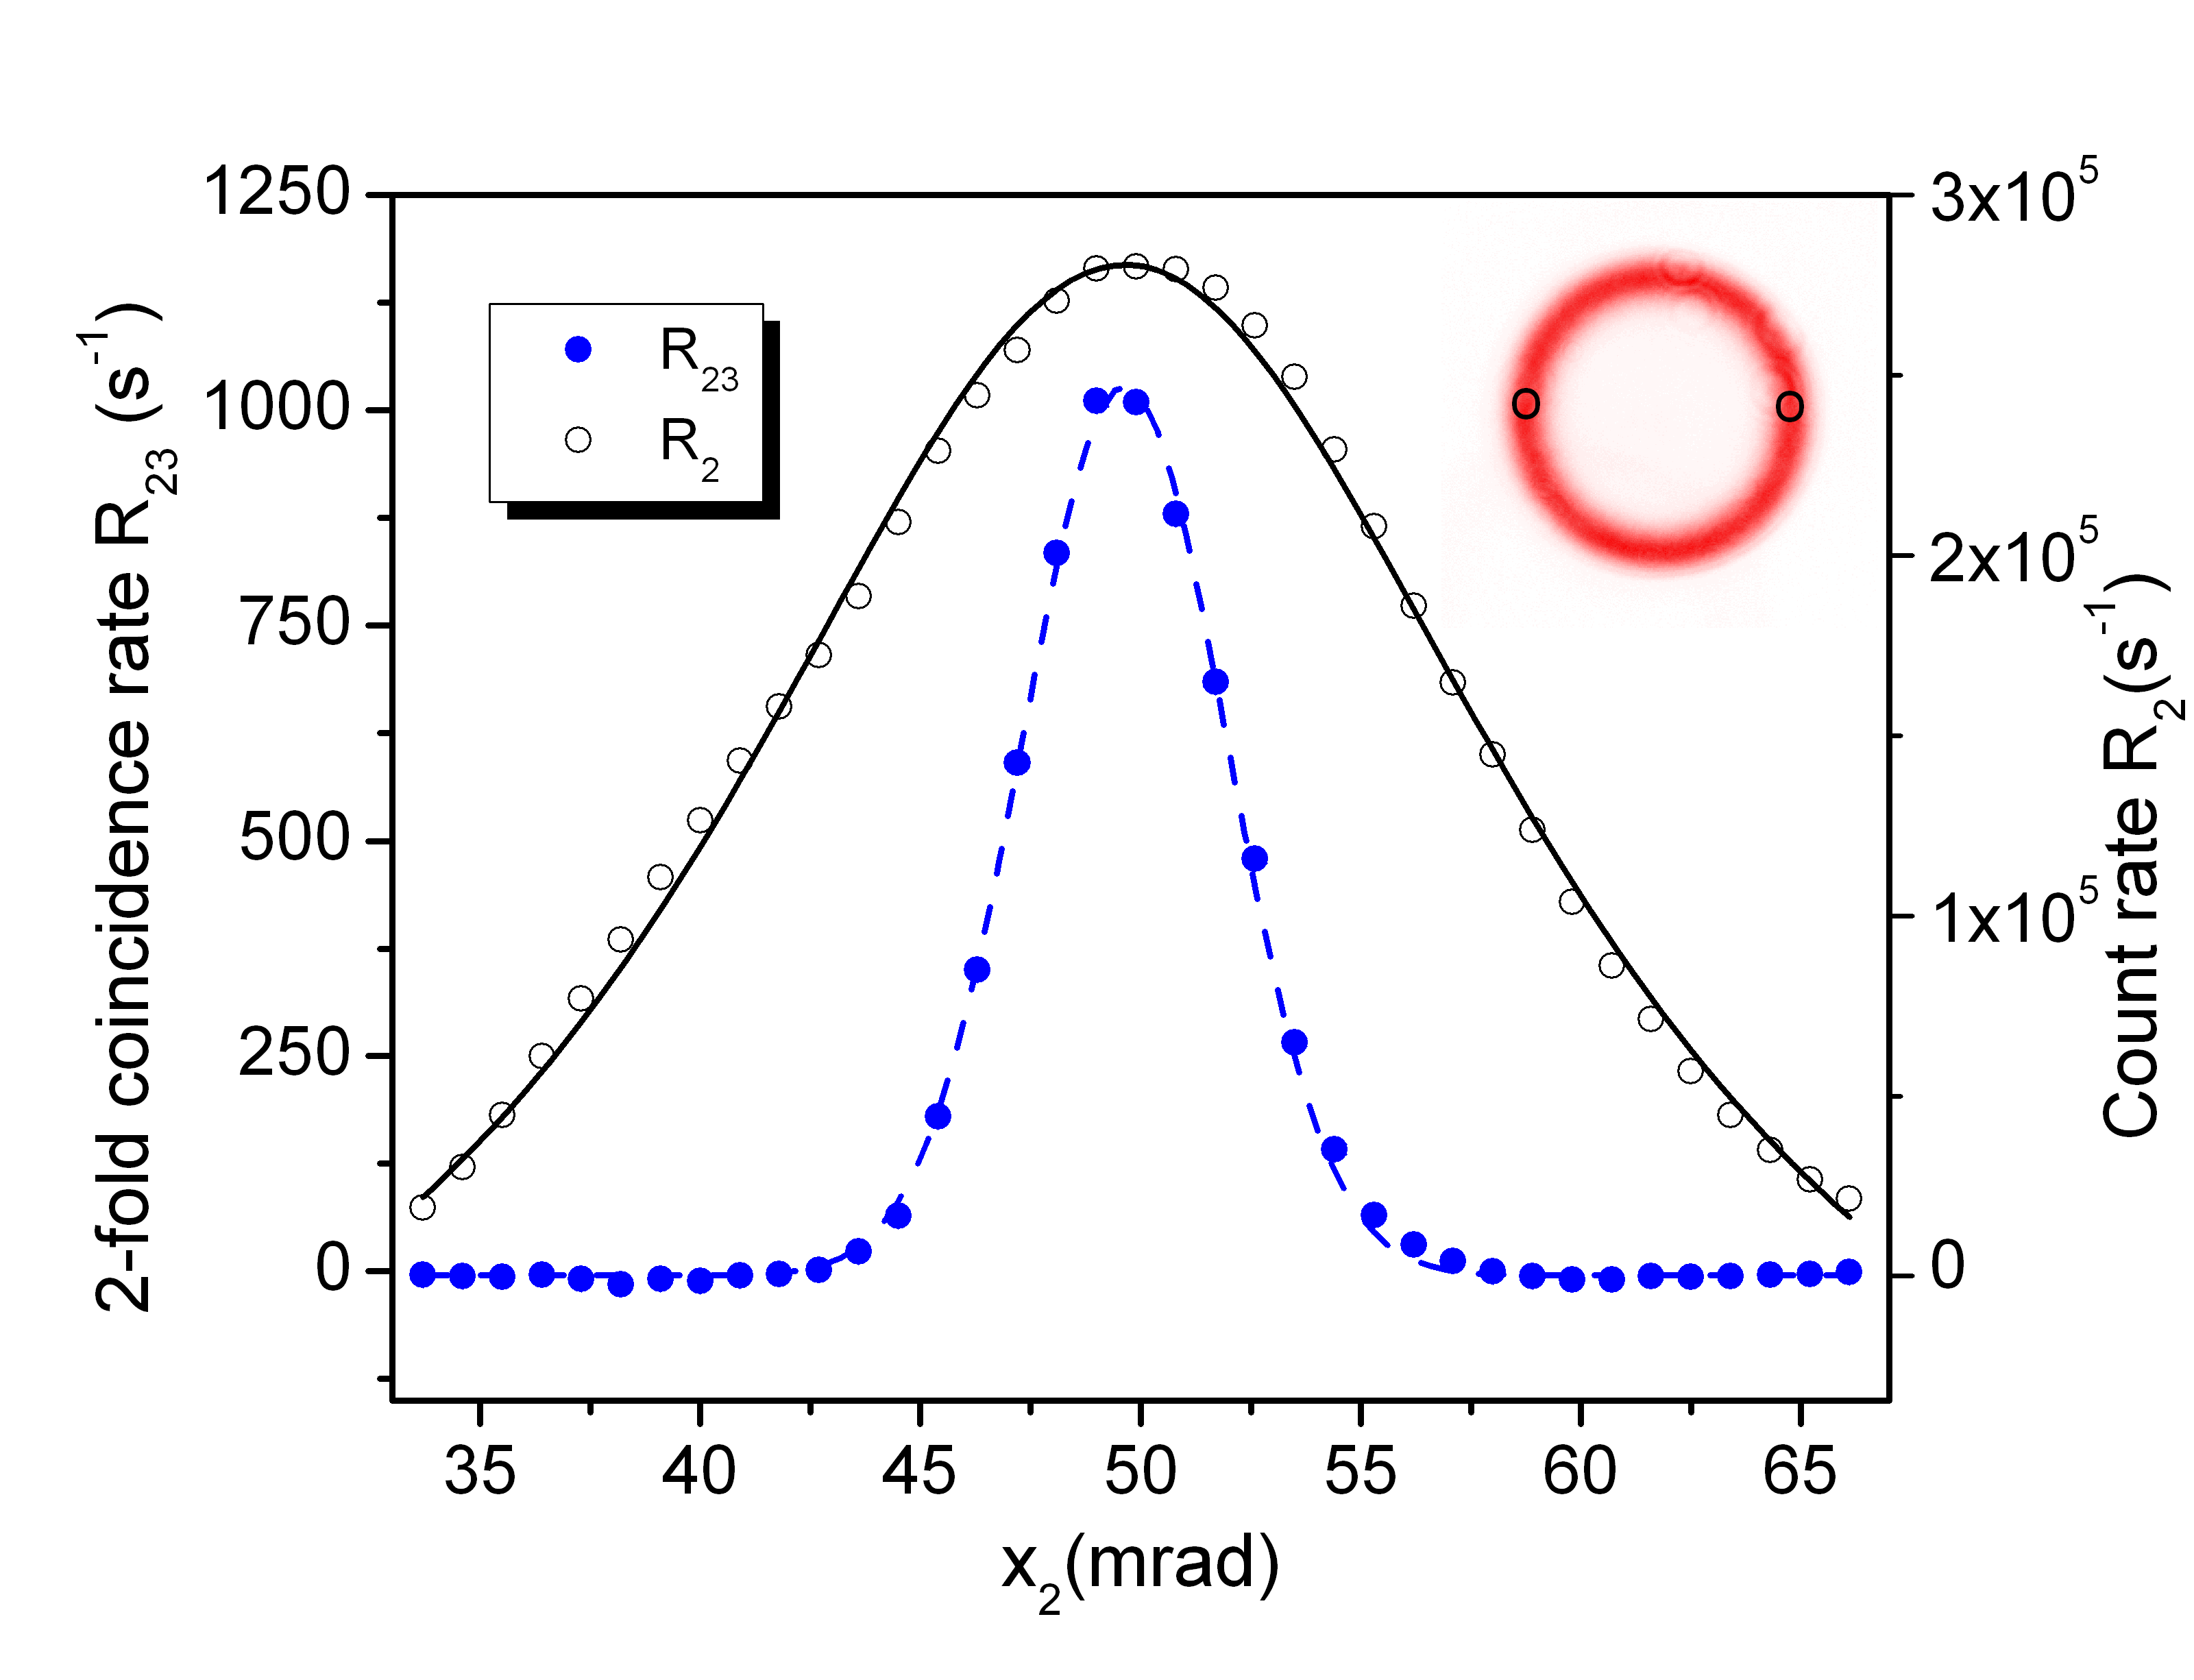
\includegraphics[width=120mm]{Fig2.png}
\caption{(Color online) Measured single count rates $R_2$ (open symbols) and 2-fold coincidence rates $R_{23}$ (filled symbols) as a function of position $x_2$, demonstrating spatial correlations in the two-photon field. The pulsed laser beam was focused in the center of the crystal using a $f$~=~250~mm lens. Data are collected using a 1 nm FWHM bandpass filter and a 1.5~mm aperture in the far-field. The solid and dashed lines indicate Lorentzian and Gaussian fits to the single and coincidence rates, respectively. The inset shows a far field image of the SPDC light emitted by the PPKTP crystal at a temperature of 20~$^\circ$C. The approximate positions of detectors D2 and D3 are shown by circles on the ring.} \label{Fig:2photons}
\end{figure}

Figure~\ref{Fig:2photons} shows the measured coincidence rate between detectors $D2$ and $D3$ (solid symbols, left axis) as a function of the position $x_2$ of detector $D_2$. Detector assembly $D_3$ is positioned at a fixed position and collects photons at an angle of -50 mrad in the far-field of the source. The measured coincidences, corrected for accidental events, are compared to the measured single count rate on detector $D2$ (open symbols, right axis). The measured single count rate on detector $D_3$ is $\sim3\cdot10^{5}$~$s^{-1}$ and is constant throughout the experiment.

The single count rate as a function of detector position is well described by a Lorentzian fit (solid line) centered at a position of 50$\pm$5~mrad and a width of 14.9$\pm$0.5~mrad FWHM. Please note that the uncertainty in the stated center position is due to the fact that it is difficult to determine the absolute position of lens $L2$ on the optical table. The characteristic minima of the $\mathrm{sinc}^2$ phase-matching curve commonly observed under continuous wave pumping are 'averaged' out by the multiple frequencies available in the spectrum of the picosecond pulsed laser~\cite{Keller1997}. The measured two-fold coincidence rate as a function of the position $x_2$ of the detector is well described by a Gaussian (dashed line) with a width (FWHM) of 5.1$\pm$0.1~mrad, and a center position of 50$\pm$5~mrad. The observation that the peak in coincidence rate is much narrower than the measured singles is a clear signature of two-photon correlations in a high-dimensional Hilbert space. The ratio of the width of the singles versus the coincidences is a direct measure of the Schmidt number $K_r$ of the (radial) spatial entanglement generated in the PPKTP crystal~\cite{DiLorenzoPires2009}. Based on the measured width of the coincidence and singles peak, we estimate a Schmidt number $K_{exp}$~$\approx$~2.9$\pm$0.1 for the pulsed laser. This estimate should be converted to a two-dimensional Schmidt number in order to compare this number to values given in literature for continuous wave pumping.

To this end, we introduce a second azimuthal Schmidt number $K_\phi$, being the ratio of the circumference of the SPDC ring, i.e. 2$\pi \times$50~mrad, over the measured width of the coincidence peak. This results in $K_\phi$~$\approx$60$\pm$6 and a corresponding Schmidt number $K$~=~$K_r K_\phi$~$\approx$~175$\pm$20. This number should be compared to calculated values~\cite{Law2004} and experimental values obtained for a 5.0~mm crystal pumped by a continuous wave laser~\cite{DiLorenzoPires2009}. The value of $K$ from ref.~\cite{DiLorenzoPires2009} for strongly negative phase mismatch (i.e. an open SPDC ring) was scaled to our case by taking into account the differences in pump beam waist and crystal length. Based on this, we expect a two-dimensional Schmidt number of $\sim$125. This value is somewhat lower than the value stated above, which we attribute to the fact that we neglected the effect of the pulsed laser on the width of the SPDC ring. The pulsed laser contains many pump frequencies which gives a slightly broader ring and consequently causes an overestimate of the value of $K_r$.

\subsection{Observation of quantum correlations of 4-photon states in the spatial degrees of freedom}

To explore the contribution of stimulated emission we measure the coincidence rate $R_{21}$ between detectors $D1$ and $D2$. Coincidences can only be registered if at least four photons are generated by a single photon pulse, since only one-photon in each pair produced by SPDC can be detected. The measured coincidence rate for photons originating from the same pulse contains both stimulated and spontaneous events. To get a measure of the number of coincidences due to spontaneous emission we introduce a tunable electronic delay between detectors $D1$ and $D2$. This allows a measurement of the coincidences in the same laser pulse ($R_{21}^{0\mathrm{ns}}$) as well as the coincidence events between subsequent laser pulses by setting the electronic delay to 12~ns ($R_{21}^{12\mathrm{ns}}$). This latter coincidence rate is dominated by events where a single pair is produced in each of the laser pulses and the coincidence rate $R_{21}^{12\mathrm{ns}}$ thus represents only the coincidence rate due to two spontaneously emitted photon pairs.

\begin{figure}[tbp]
\centering 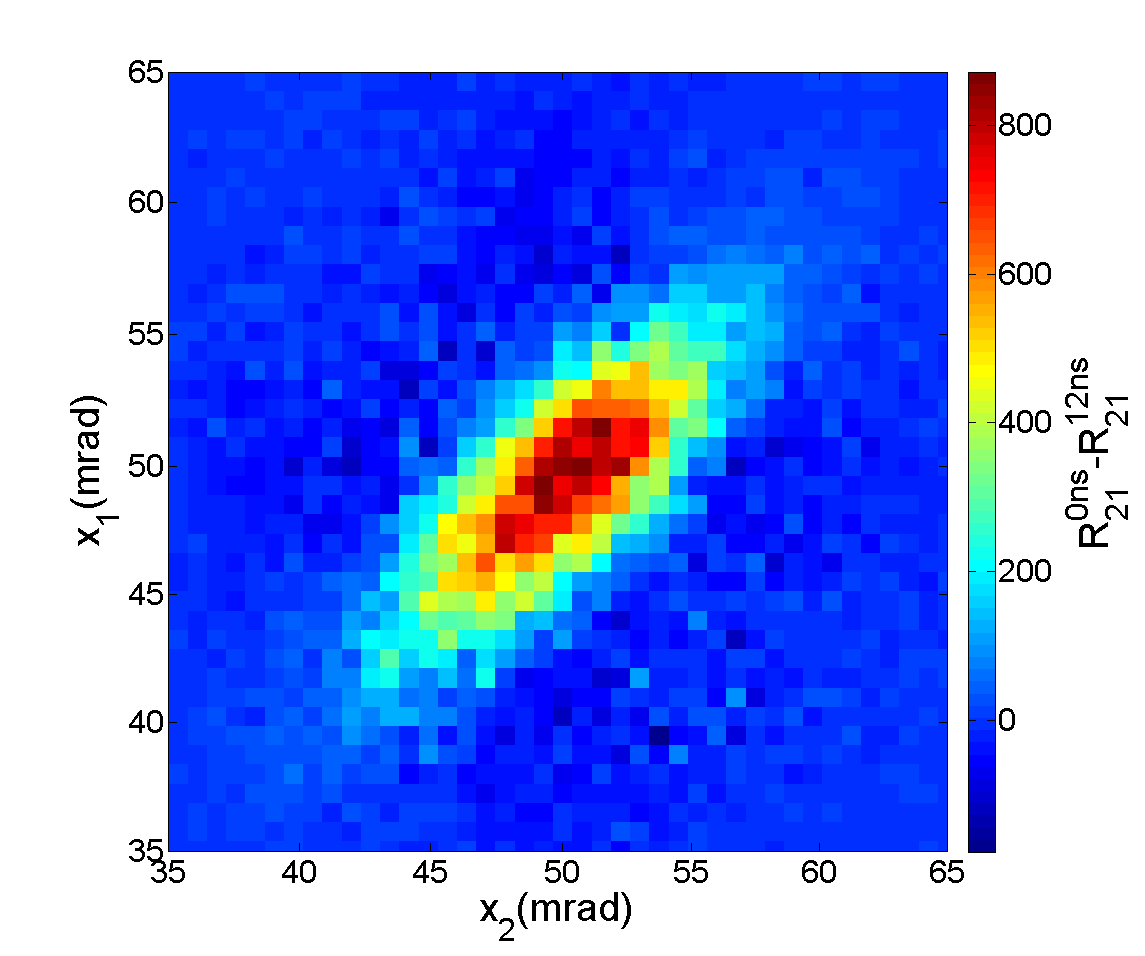
\includegraphics[width=87mm]{Fig3a.png} \\
\centering 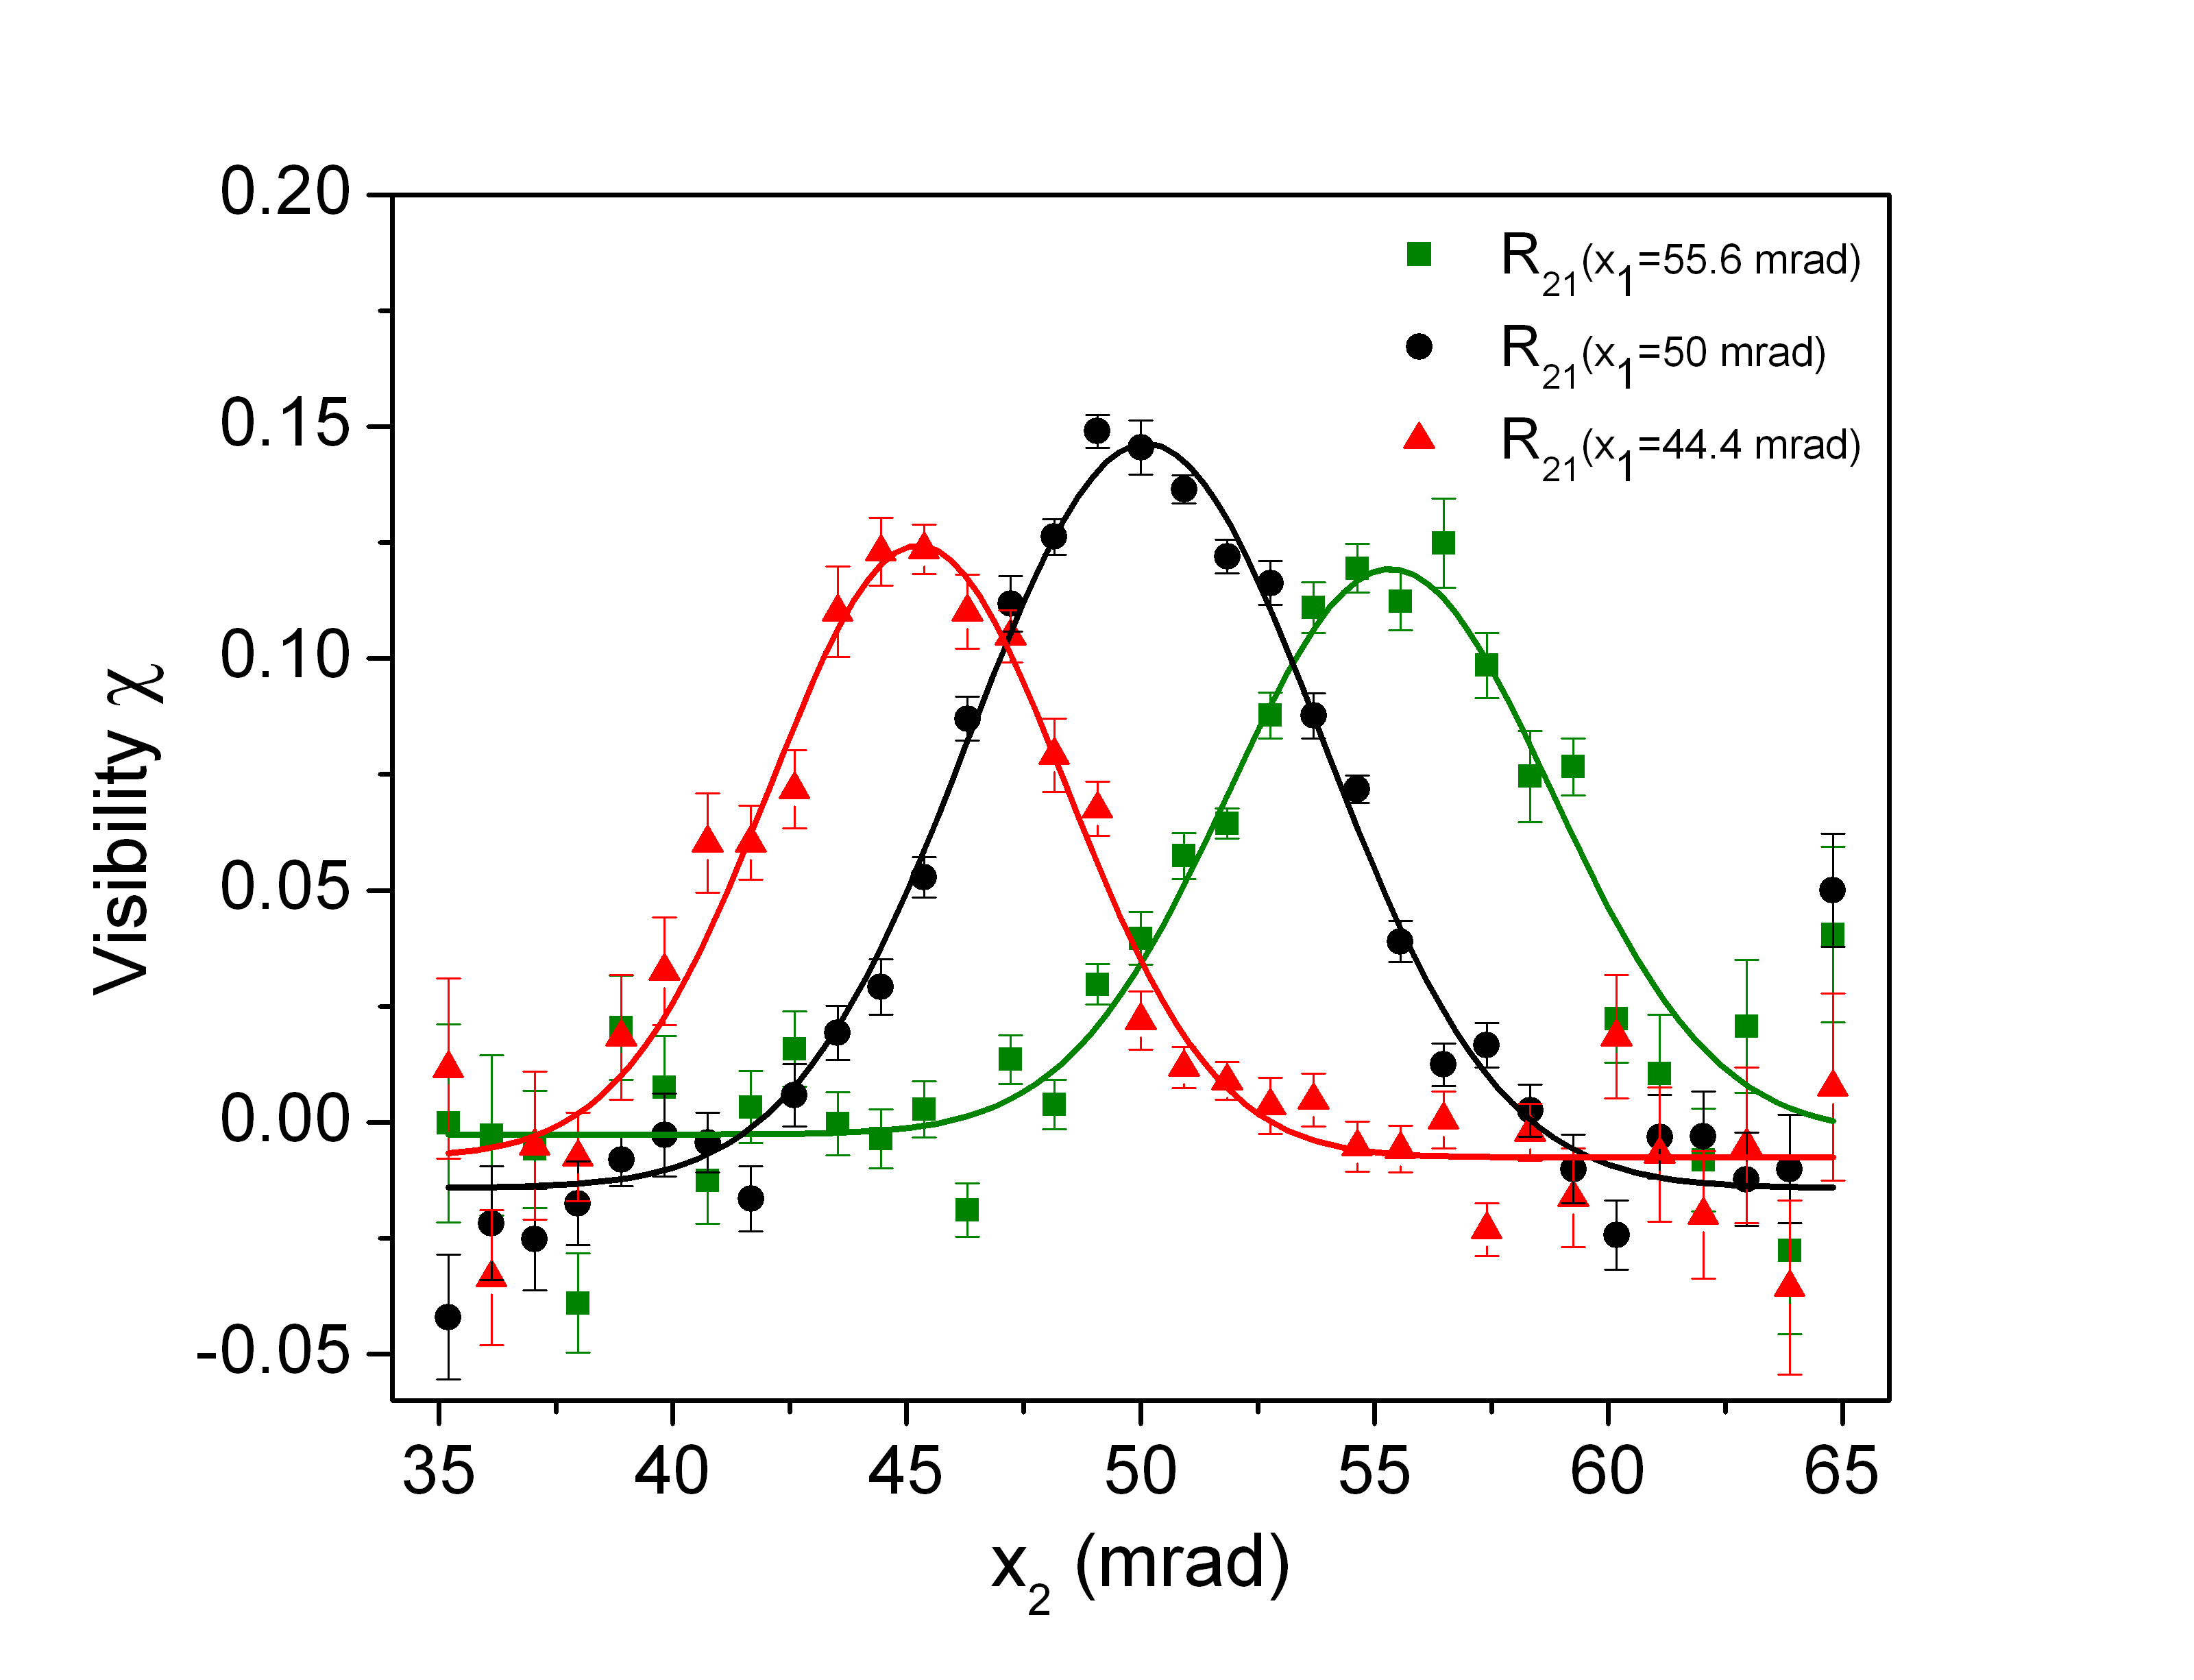
\includegraphics[width=87mm]{Fig3b.png}
\caption{(Color) Measured joint spatial distribution of stimulated pair emission. (a) False-color plot of the measured difference in coincidence rate $(R_{21}^{0\mathrm{ns}} - R_{21}^{12\mathrm{ns}})$  as a function of the positions of $x_1$ and $x_2$ of detectors $D_1$ and $D_2$. Data are collected with a 5~nm FWHM bandpass filter and a 1.5~mm aperture size. The observed maximum coincidence rate $(R_{21}^{0\mathrm{ns}}$ is typically 25,000~s$^{-1}$. The data clearly demonstrate that stimulated pair emission occurs when the photons are emitted in the same spatial mode, i.e. when $x_1$~=~$x_2$. (b) Visibility $\chi$ of the 4-photon state as a function of position $x_2$. The different symbols (triangles, circles, squares) correspond to different positions $x_1$ (44.4, 50.0, 55.6~mrad) of detector $D_1$. Data are collected using a 1~nm FWHM bandpass filter and a 1.5 mm aperture. The solid lines through the data are Gaussian fits.}\label{Fig:4photon}
\end{figure}

The difference in these coincidence rates, normalized by the coincidence rate due to spontaneous events is equal to the ``visibility'' $\chi$, i.e. $\chi = (R_{21}^{0\mathrm{ns}} - R_{21}^{12\mathrm{ns}})/R_{21}^{12\mathrm{ns}}$ and is a good measure of the extra events due to stimulated emission of 4-photon states. The measured visibility as a function of the position of the two detectors, $\chi(x_1,x_2)$, can be interpreted as a joint spatial density of stimulated pair emission. This joint spatial distribution of stimulated pair emission is depicted in Fig~\ref{Fig:4photon}. The false colour image in Fig.~\ref{Fig:4photon}a shows the difference in coincidence rate $(R_{21}^{0\mathrm{ns}} - R_{21}^{12\mathrm{ns}})$ as a function of the position $x_1$ and $x_2$ of detectors $D1$ and $D_2$ using a 5~nm bandpass filter for the SPDC light. The image is centered around the point $x_1$~=~$x_2$~=~50~mrad and clearly shows the expected positive correlation due to stimualted emission of the 4-photon state that leads to extra coincidences whenever the two detectors detect photons in the same optical mode, i.e. when $x_1$~=~$x_2$. The width (FWHM) of the peak along the diagonal ($x_1-x_2$~=~0~mrad) is 11.5$\pm$0.3 mrad, while the width along the anti-diagonal direction ($x_1+x_2$~=~100~mrad) is 4.5$\pm$0.1 mrad.

Figure~\ref{Fig:4photon}b shows the visibility $\chi(x_1,x_2)$ as a function of position $x_2$ of detector $D2$ for a fixed position of detector $D1$. The three curves correspond to $x_1$~=~44.4~mrad (triangles), 50.0~mrad (circles) and 55.6~mrad (squares). These data are taken with a 1~nm bandpass filter for the SPDC light in order to enhance the visibility at the expense of a much lower count rate. The narrow band frequency filter lowers the number of temporal modes involved, but does not affect the spatial modes. The integration time per point was increased by repeated scanning of the detector in the $x_2$ direction. Because the phase-mismatch of the PPKTP crystal that governs the SPDC process depends weakly on laser power, the long term stability of the laser becomes important. In order to correct for this effect we also monitor the single counts on the detector $D2$ as a function of position $x_2$ and exclude scans from our analysis where the SPDC ring appears shifted. The solid lines through the data are Gaussian fits to the data with a FWHM width of 8.9$\pm$0.3. The peak positions are shifted to the position of detector $D1$, such that the peak of the Gaussian appears at $x_1$~=~$x_2$. The obtained peak visibilities for the three curves are 0.13$\pm$0.01, 0.16$\pm$0.01 and 0.12$\pm$0.01. For a uniform illumination of the aperture one would expect the peak visibility to be independent of the position $x_1$. This case corresponds to a situation where the width of the SPDC ring, as given by the phase-matching function, is much larger than the shift in position $x_1$. In our experiment the slightly lower visibility for $x_1$~=~44.4 and 55.6~mrad is caused by the finite diameter of the 1.5~mm aperture that captures a non-uniform part of the SPDC ring. For larger apertures (data not shown) this decrease in visibility indeed becomes more significant.

The visibility in our experiment is limited by both the number of temporal modes collected as well as by the ratio of the total number of spatial modes available over the number of spatial modes collected by the aperture. The total number of temporal modes generated is given by the frequency bandwidth of the SPDC light as compared to the frequency spread of the pulse. For a Fourier limited pulse shape the frequency bandwidth is related to the pulse duration via $\tau = (2 \ln(2) \lambda^2)/(/\pi c \Delta \lambda)$, where $\tau$ is the pulse duration and $\lambda/\Delta \lambda$ is the relative frequency spread. The 2~ps pulse corresponds to an equivalent spectral width of 0.5~nm, while the 2~mm PPKTP crystal produces SPDC light with a bandwidth of $\sim$40 nm FWHM. Consequently, the number of available temporal modes for a PPKTP crystal pumped by a 2~ps laser is pulse is potentially $\sim$80. We use '5 nm' and '1 nm' bandpass filters centered at 826.4 nm to limit the number of temporal modes. The measured FWHM bandwidth of these filters is 4.6~nm and 1.5~nm, which extends the coherence time of the SPDC light and limit the number of temporal modes to $\sim$9 and $\sim$3 respectively. Since $\chi$ is inversely proportional to the number of available temporal modes~\cite{Riedmatten2004}, this produces upper limits to $\chi$ of 0.1 and 0.3 for the two bandpass filters. We stress that shorter pump pulses do not necessarily lead to a higher flux of photons since the phase-matching in the 2~mm PPKTP crystal effectively filters the pump pulse. In our experiments we have carefully chosen the crystal length to maximize conversion efficiency without significantly stretching the pump pulse to avoid a non-factorable structure ('X-entanglement') between spatial and temporal degrees of freedom~\cite{Gatti:PRL2009}.

\begin{figure}[tbp]
\centering 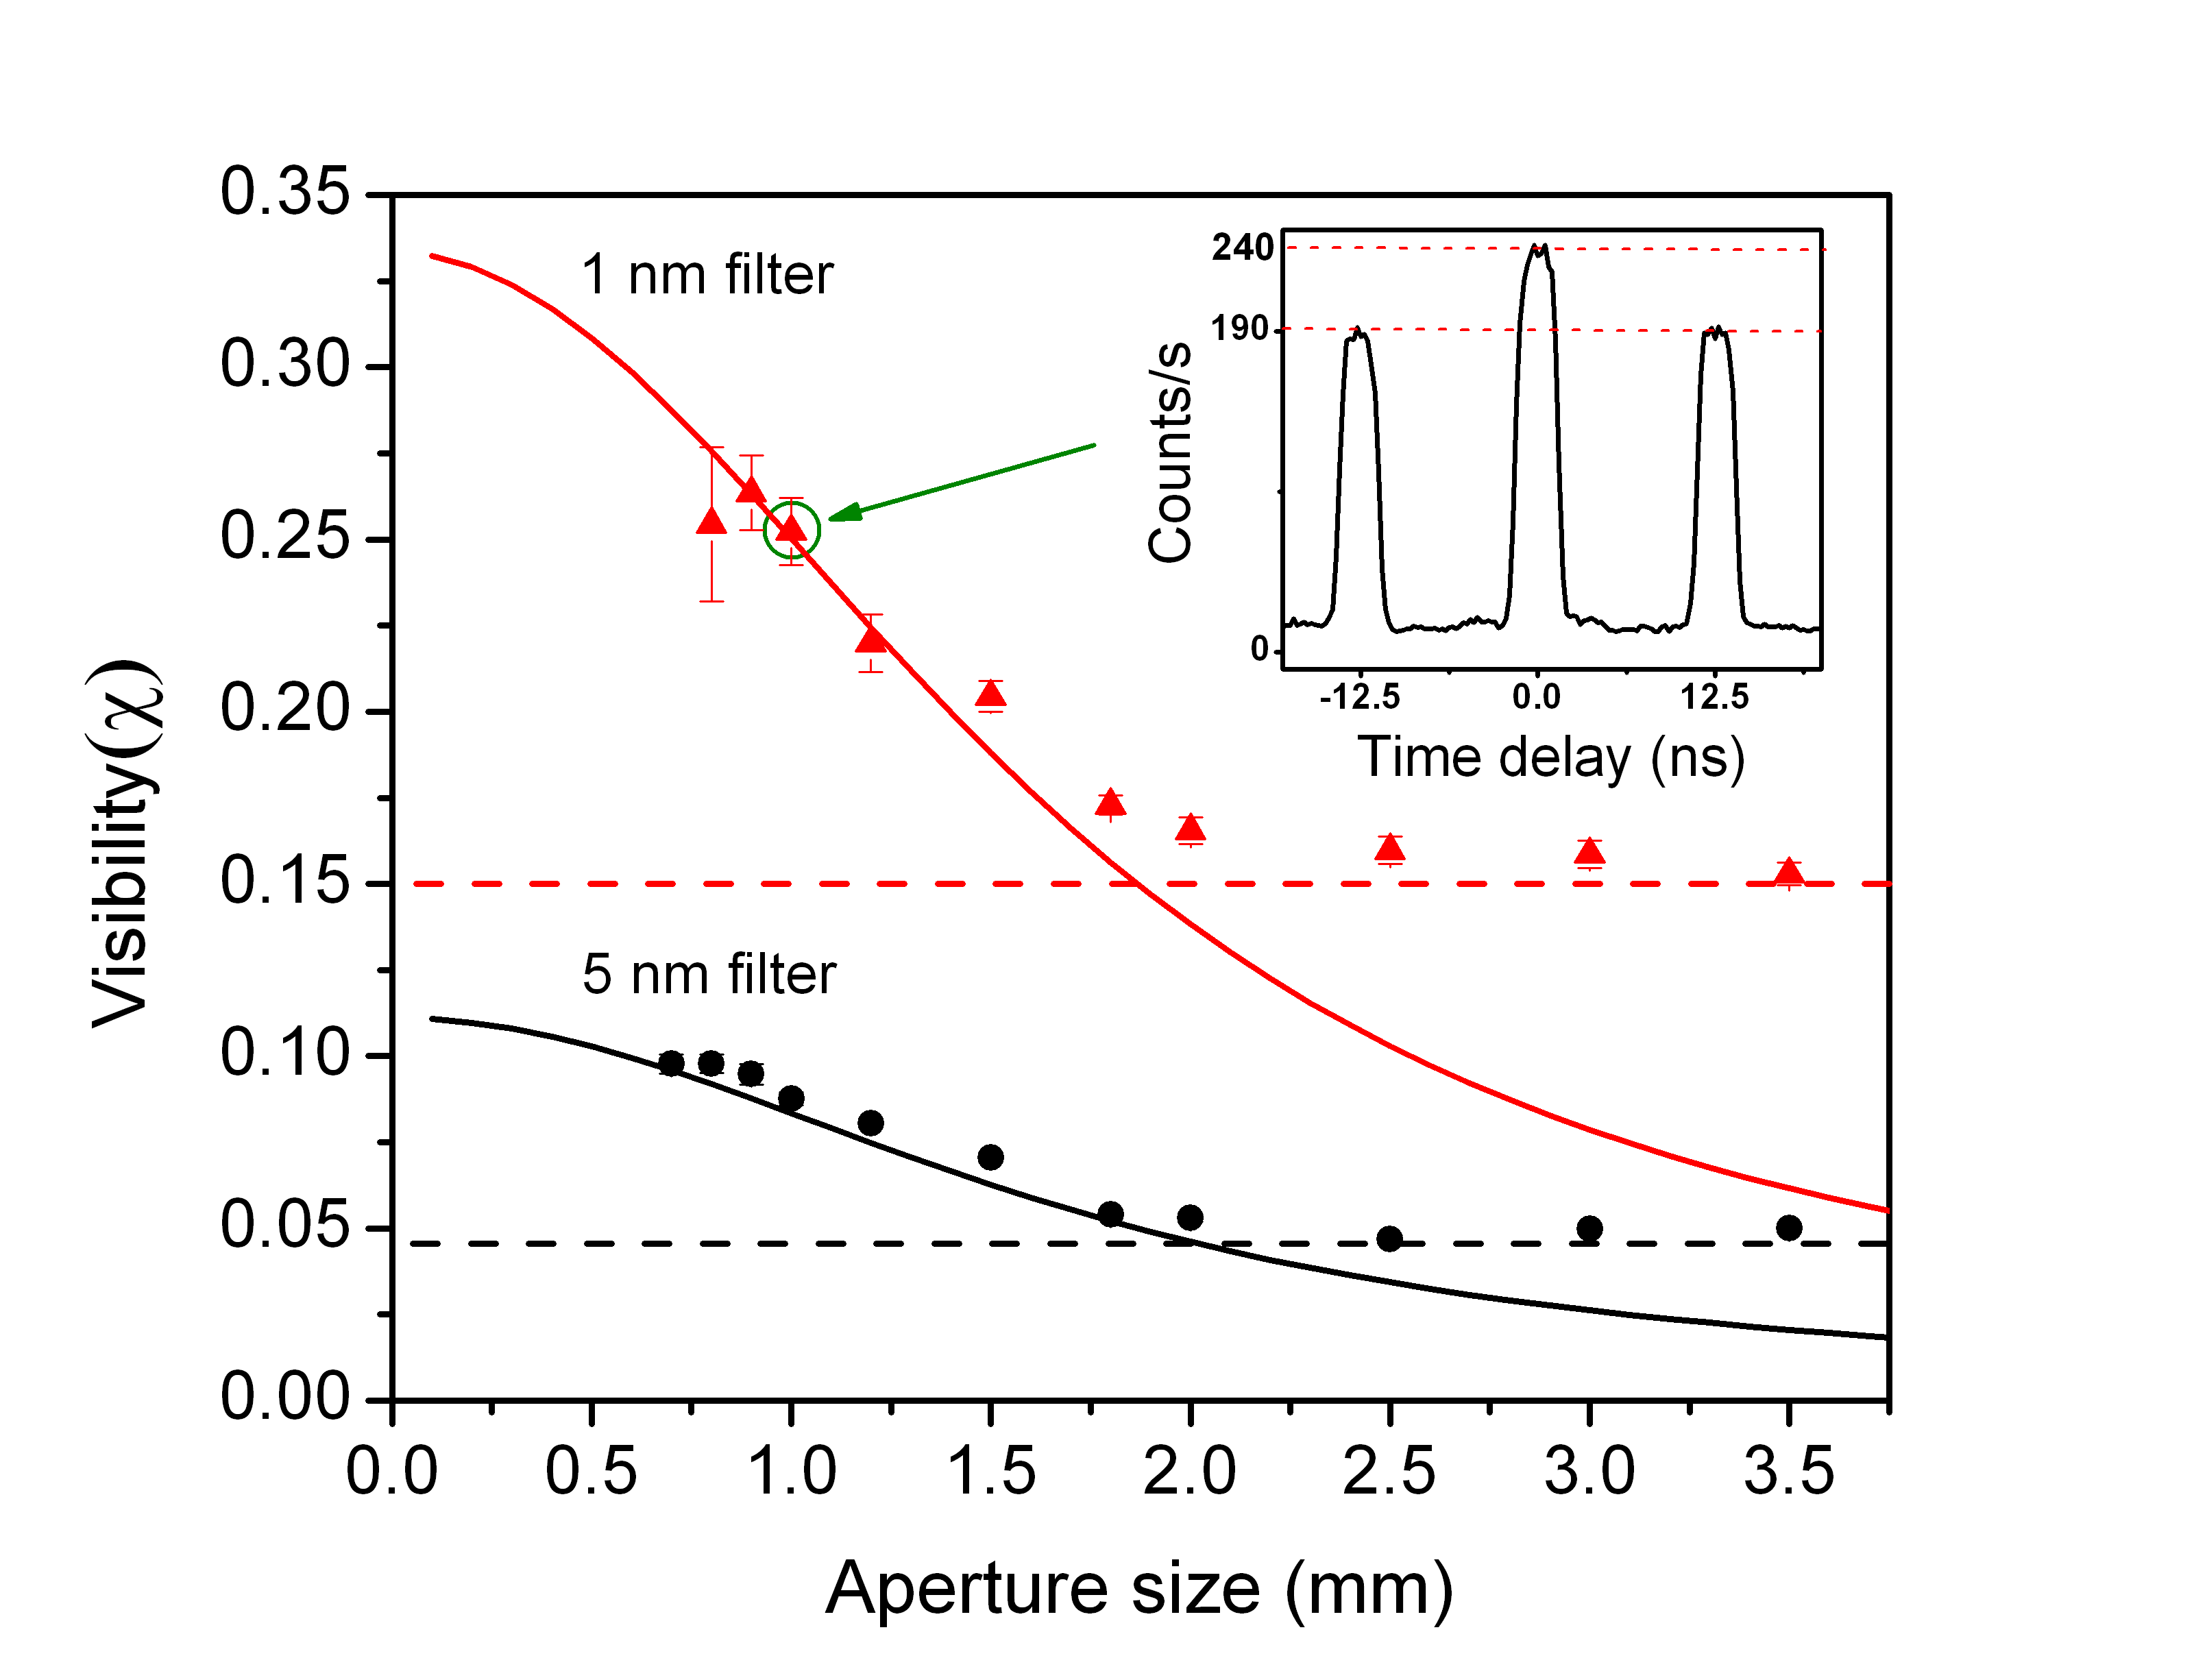
\includegraphics[width=87mm]{Fig4.png}
\caption{(Color online) Visibility $\chi$ of the 4-photon state as a function of aperture size using a 1~nm FWHM bandpass filter (triangles) and a 5~nm FWHM bandpass filter (circles). These data are obtained by subtracting the measured coincidence rate at a delay of 12~ns from the measured coincidence rate at zero delay. Typical single count rates on the detector are $1.4\times10^6$ and $3\times10^5$ sec$^{-1}$ for apertures $>$ 2 mm and drop to $5\times10^5$ and $1\times10^5$ sec$^{-1}$ for a 1 mm aperture size. The solid lines represent a calculation with no free parameters (see text). For apertures larger than 2 mm, the aperture is limited by lens $L3$ and the numerical aperture of the fiber and the visibility saturates as indicated by the horizontal dashed lines. The inset shows the measured coincidence rate $R_{12}$ as a function of electronic delay for a 1~nm FWHM bandpass filter and a 1~mm aperture size ($\chi$~=~0.25), indicated by the arrow.}\label{Fig:Visibility}
\end{figure}

Figure~\ref{Fig:Visibility} shows the measured visibility as a function of aperture size for a 5~nm bandpass filter (circles) as compared to a 1~nm bandpass filter (triangles). Measurements were performed by measuring coincidence rates between detectors $D1$ and $D2$ at a fixed position $x_1$~=~$x_2$~=~50~mrad. A measurement of the coincidence rate as a function of the electronic time delay is shown in the inset for a point with a relatively high visibility of 0.25. The extra 50 counts/sec at zero delay are due to stimulated emission of photon pairs. Clearly, the visibility is low and nearly constant for apertures that are larger than 2~mm and rises as the number of available spatial modes is reduced by closing the aperture. In our experiments the visibility saturates at apertures sizes above 2 mm where the apertures size is limited by the finite numerical aperture of the multimode fiber in combination with the focal length of the fiber coupling lens $L3$. The saturation is represented by the horizontal dashed lines.

The visibility $\chi$ in the experiment is proportional to the inverse of the number of spatial and temporal modes, i.e. $\chi \propto N_t^{-1} N_{sp}^{-1}$, where $N_t$ and $N_{sp}$ are the number of temporal and spatial modes respectively. Throughout the experiment $N_t$ is determined by the FWHM of the bandpass filter and can be considered constant. We use values of $N_t$ = 9 and $N_t$ = 3 for the two different bandpass filters. In order to estimate the number of spatial modes collected as a function of aperture size we consider the correlations between two point-like apertures at positions $\vec{r_1}$ and $\vec{r_2}$. The resulting visibility is given by:
\begin{equation}
\chi(\vec{r_1},\vec{r_2})=\exp(-\frac{|\vec{r_1}-\vec{r_2}|^2}{r_0^2}).
\end{equation}
The characteristic distance $r_0 = (\lambda f_2)/(\pi w_p)$, where $f_2$ = 270 mm is the focal distance of lens $L2$ that creates the far-field of the SPDC source and $w_p$ is the waist of the pump beam created by focussing the pump beam using lens $L1$. Using the measured waist of the pump beam of 80~$\mu$m we find a characteristic distance $r_0$~=~0.9 mm. The visibility in the experiment due to finite aperture size for two apertures centered at the same position can be found via integration:
\begin{equation}
 \chi (a) = \frac {1}{N_t \pi^2 a^4} \iint \chi(\vec{r_1},\vec{r_2}) \Theta(|\vec{r_1}|-a) \Theta(|\vec{r_2}|-a) \mathrm{d}\vec{r_1} \mathrm{d}\vec{r_2}, \label{vis}
\end{equation}
where the Heaviside step-functions $\Theta(|\vec{r_1}|-a)$ and $\Theta(|\vec{r_2}|-a)$ represent the sharp edges of the two apertures with equal radius $a$ in the far-field. The solid lines through the data in Fig.~\ref{Fig:Visibility} are the results of calculating the double integral represented by equation~\ref{vis} using 3 and 9 temporal modes for the two bandpass filters and the calculated value of $r_0$ based on the measured beam waist. The agreement between the data and the model with no adjustable parameters is striking for aperture sizes below 2 mm. For apertures above 2 mm the visibility saturates, as indicated by the horizontal dashed lines, at a value determined by lens $L3$ and the numerical aperture of the multimode fiber that limit the beam diameter to $\sim$2~mm.

\section{Conclusion}

In conclusion, we have demonstrated the existence of spatial correlations between photon pairs in a 4-photon state. These correlations are induced via stimulated pair emission. In our experiments we are able to separate the contribution from spontaneous parametric down-conversion and stimulated parametric down-conversion at the level of double pairs. The stimulated emission becomes important when a 2~mm long PPKTP crystal is pumped by a 2~ps pulsed laser at 413.2~nm wavelength to create frequency and polarization degenerate photon pairs at a wavelength of 826.4~nm. The spatial correlations of the stimulated photon pairs contains a rich structure when using a non-colinear geometry for the down-conversion process, which can be explored with relative ease using apertures in the far-field. In this way we present the first measurements of the joint spatial distribution of stimulated pair emission and discuss the acquired visibility. This technique opens new possibilities to explore the structure of higher-dimensional entanglement by making use of spatial degrees of freedom instead of the temporal degree of freedom. The possibility to distinguish between stimulated and spontaneous processes can be used to explore recent proposals for ghost imaging with thermal and quantum light sources\cite{Chan:PRA2009,Osullivan:PRA2010}.

